\begin{titlepage}
% \newgeometry{margin=1cm}
% \begin{center}
% \vspace{-3.5cm}
% \hspace{-3.5cm}
% 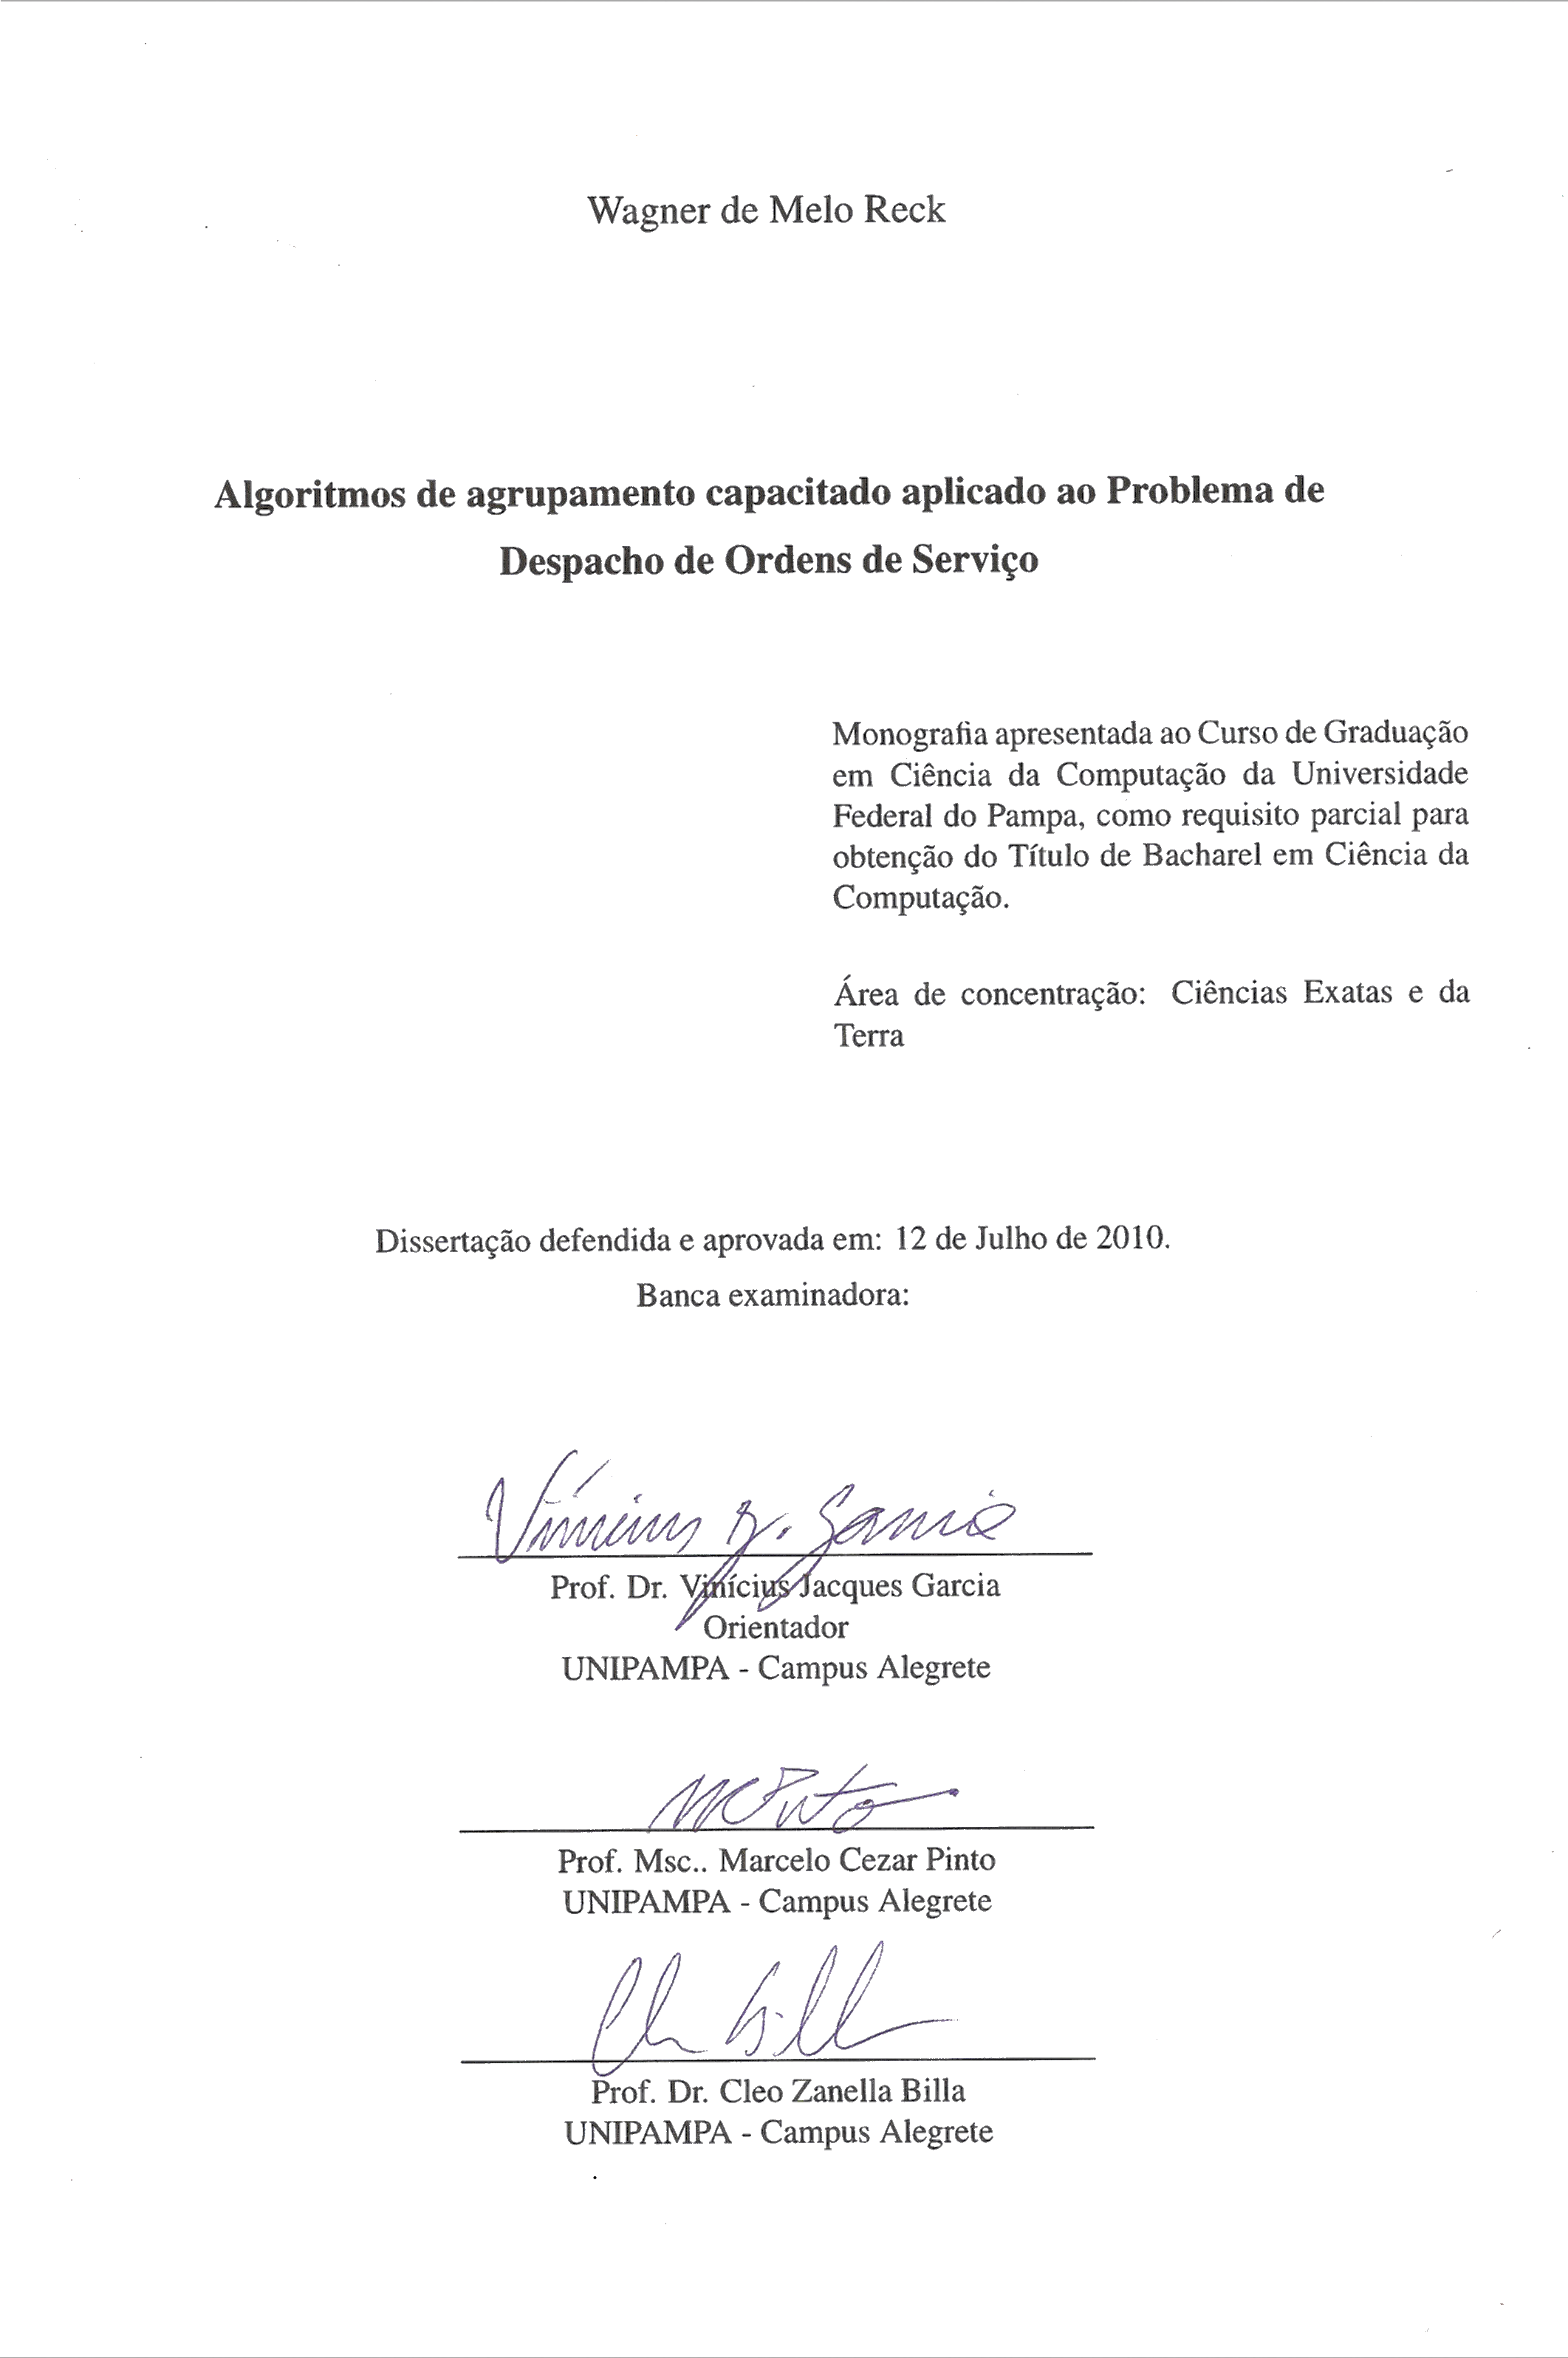
\includegraphics[width=\paperwidth,height=0.9\paperheight,
% keepaspectratio]{./images/ficha_aprovacao.png}%
% % \restoregeometry{}
% %  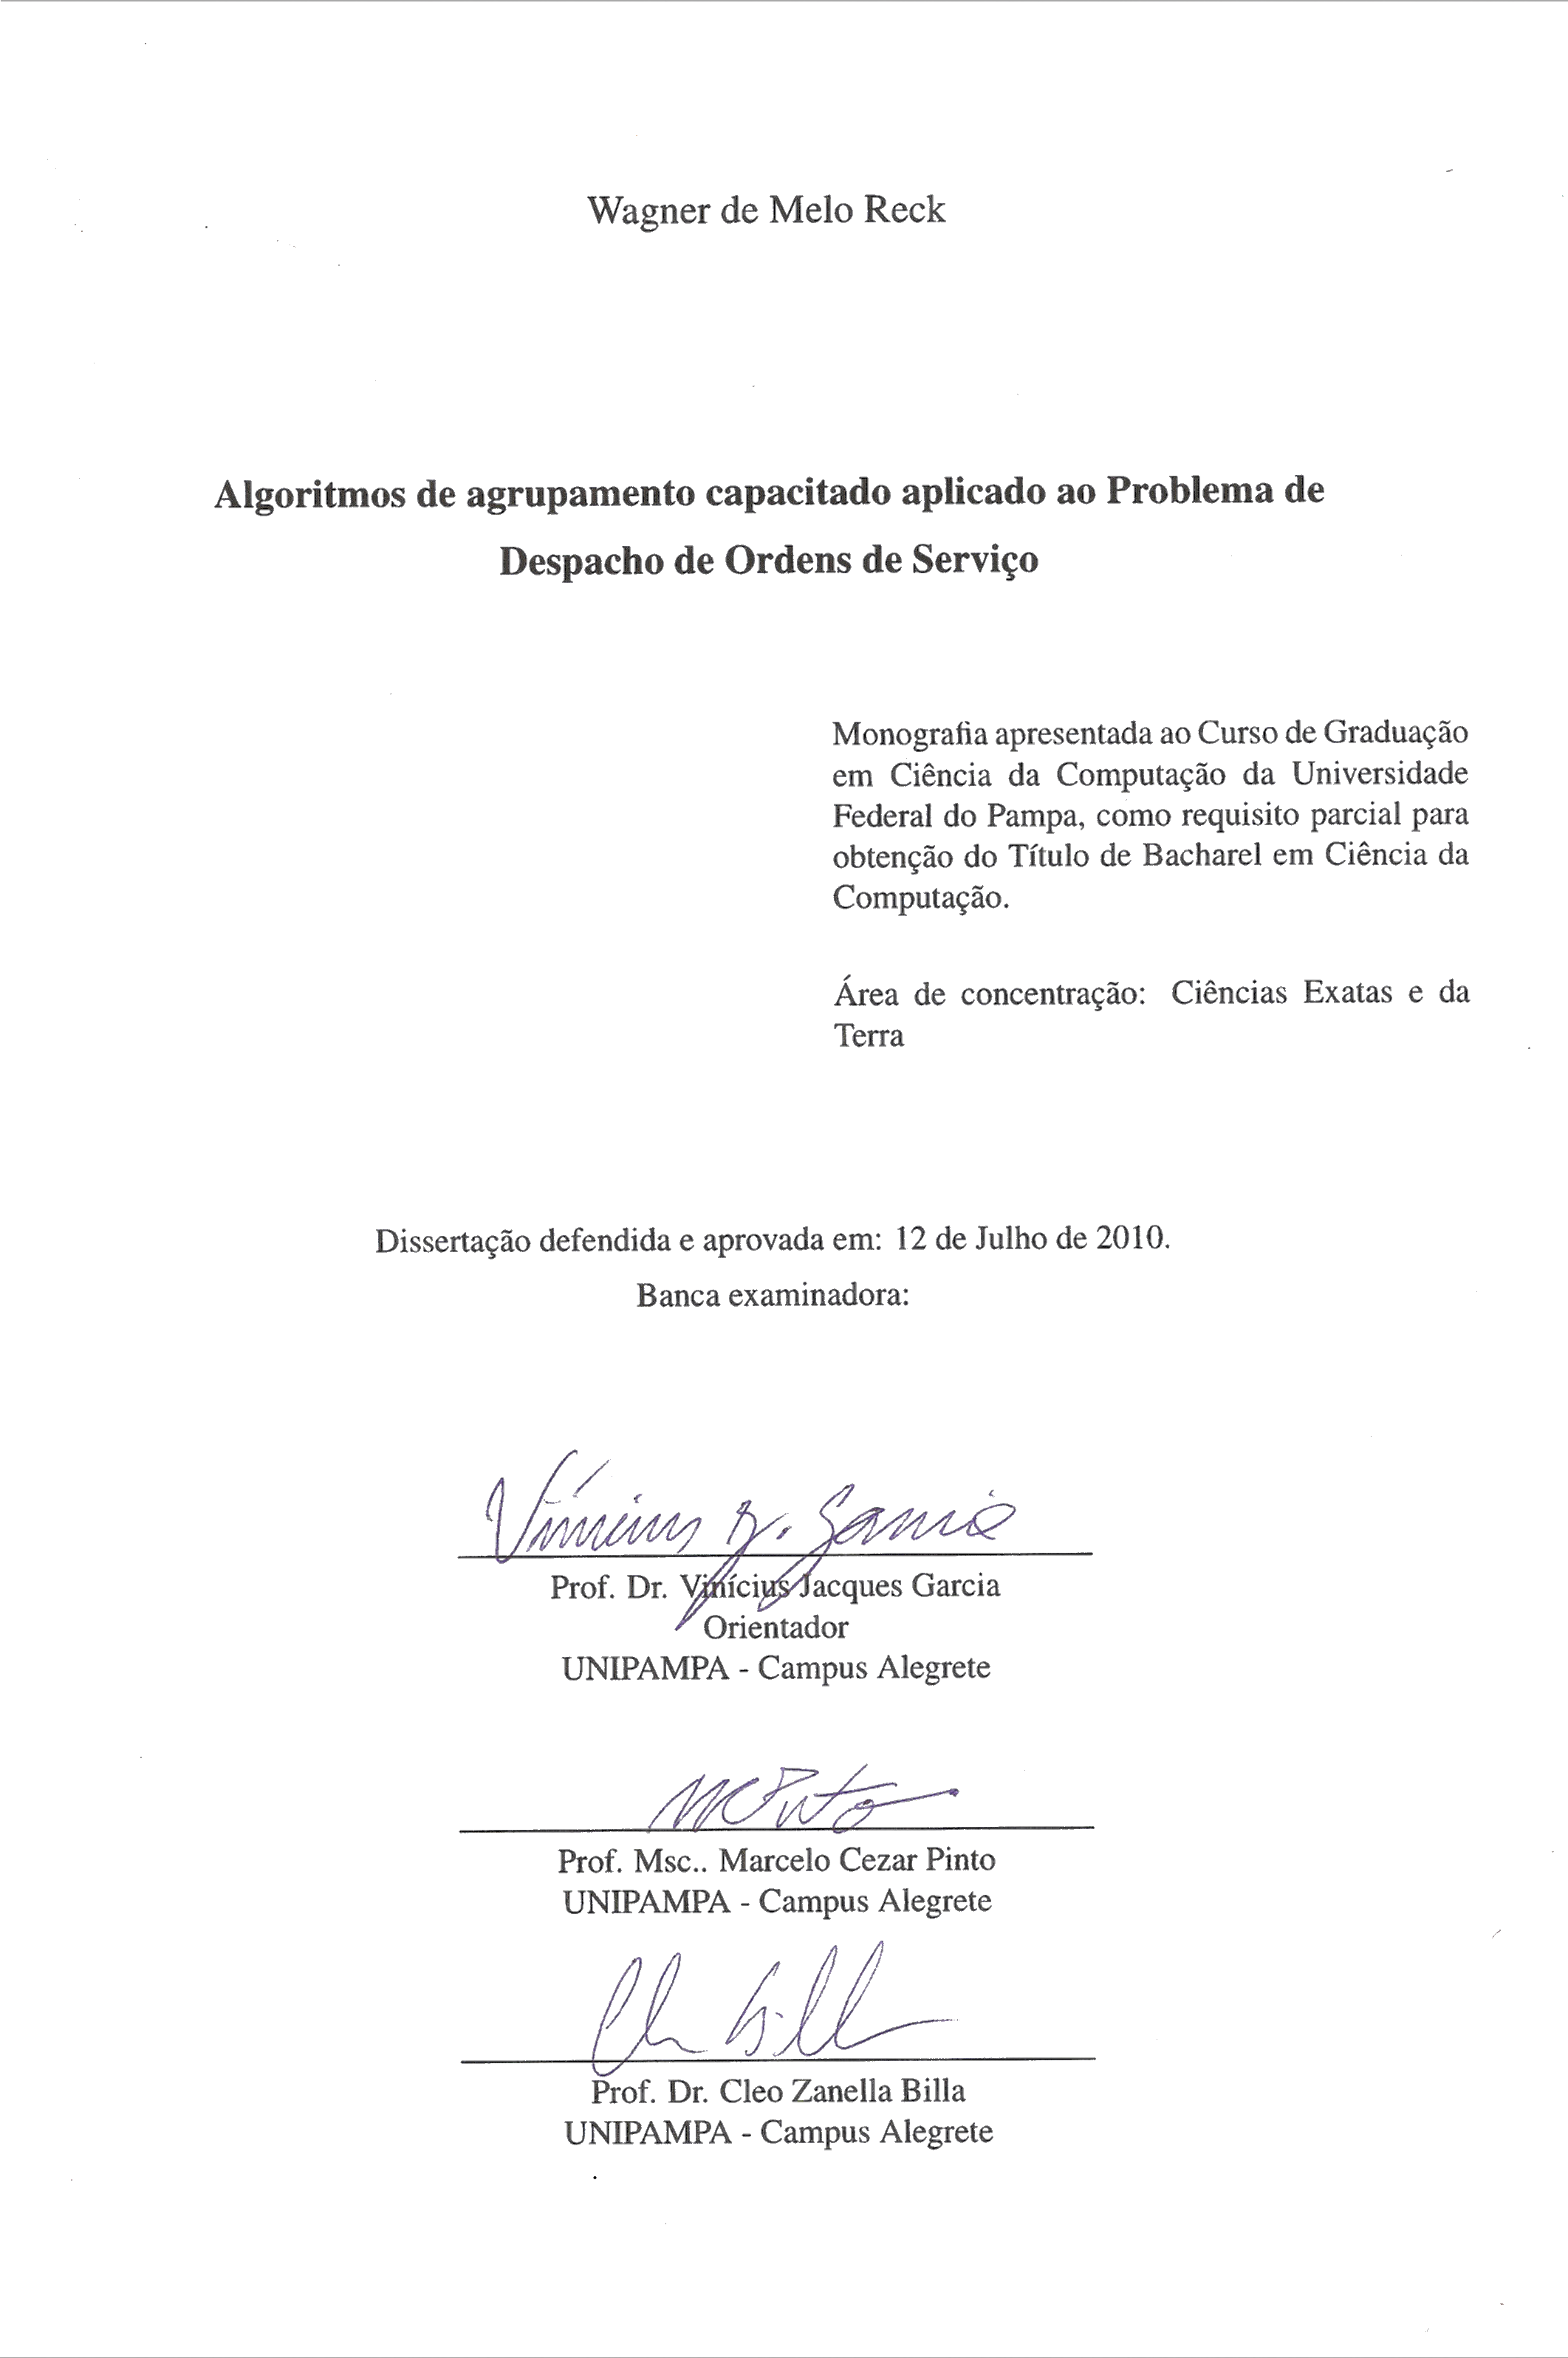
\includegraphics[scale=0.32]{./images/ficha_aprovacao.png}
% %  % ficha_aprovacao.png: 2123x3192 pixel, 96dpi, 56.16x84.44 cm, bb=0 0 1592 2394
% \end{center}
% \end{titlepage}

% \put(0,0){
% \parbox[b][\paperheight]{\paperwidth}{%
% \vfill
% \centering
% 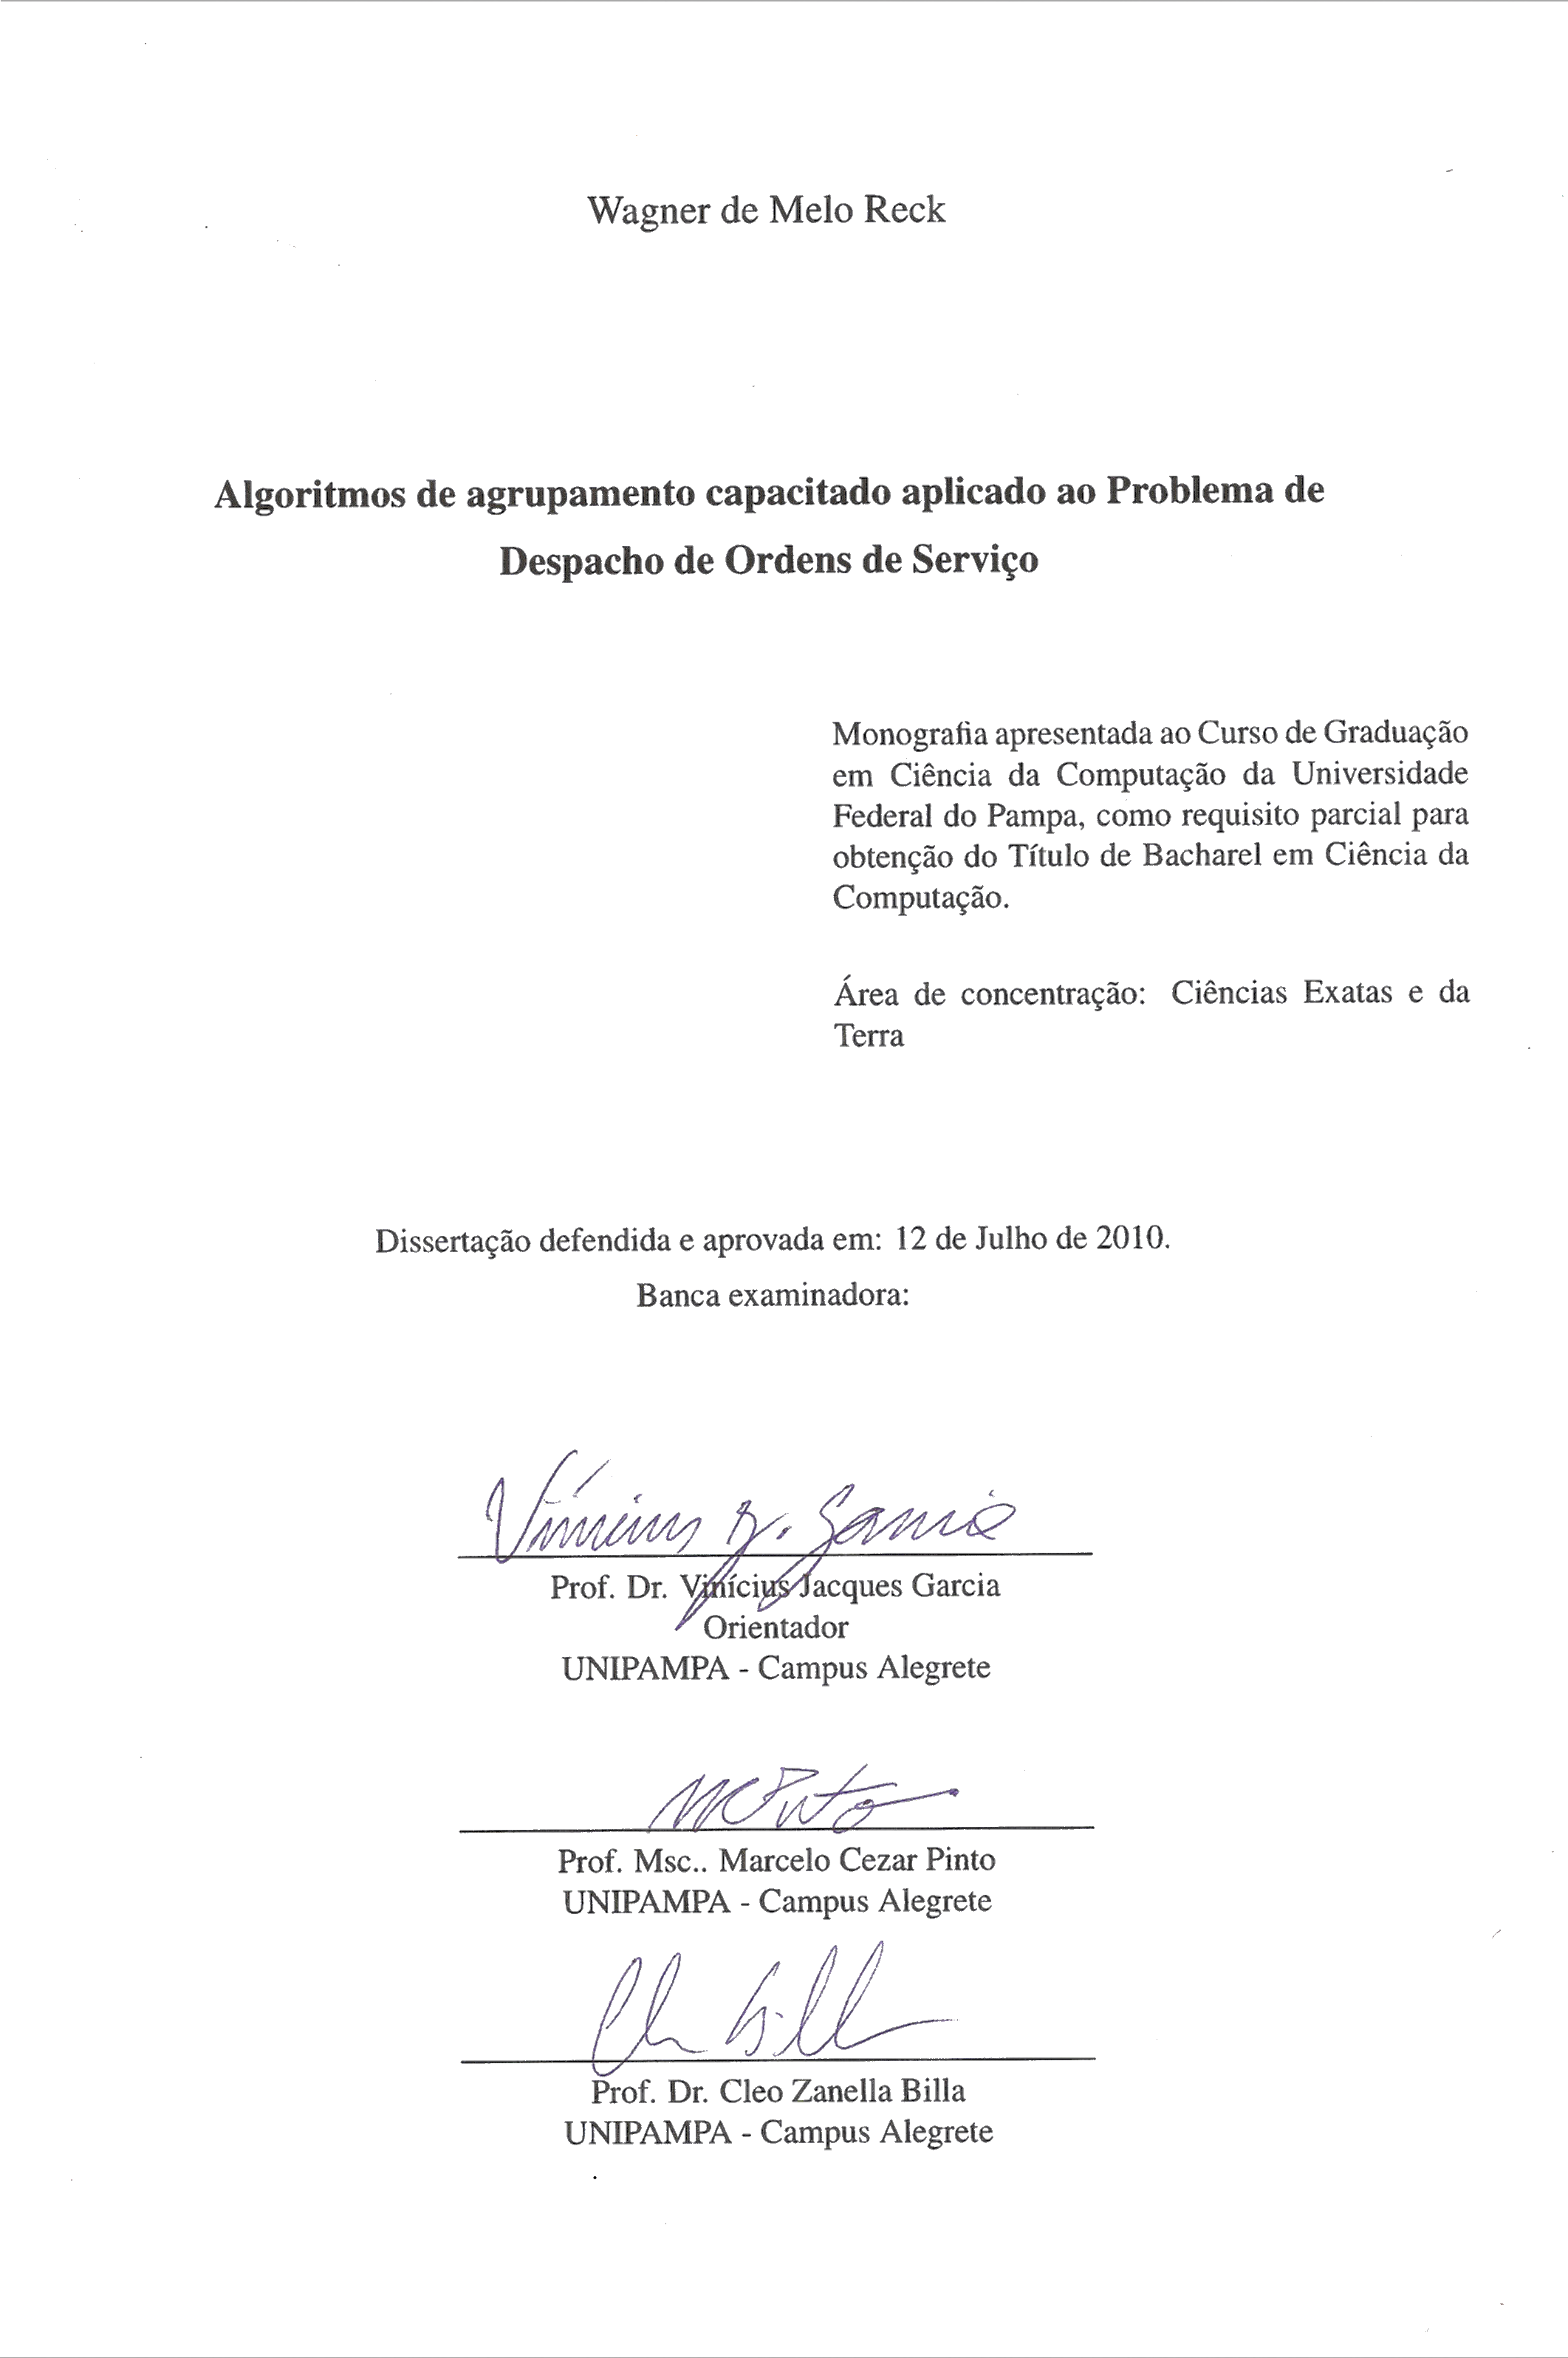
\includegraphics[width=\paperwidth,height=\paperheight,
% keepaspectratio]{./images/ficha_aprovacao.png}%
% \vfill
% }
% }

\vspace{0.75cm}

\begin{center}
	\large\ABNTautordata
\end{center}

\vspace{1.5cm}

\begin{center}
	\large\ABNTtitulodata
\end{center}

\vspace{1cm}

\hspace{8cm}
\begin{minipage}{8cm}
\begin{espacosimples}
Disserta��o apresentada ao Programa de P�s-gradua��o \textit{Strictu Sensu} em
Engenharia El�trica da Universidade
Federal do Pampa, como requisito
parcial para obten��o do T�tulo de
Mestre em Engenharia El�trica.
\vspace {0.7cm}
\\�rea de concentra��o: Ci�ncias Exatas e da Terra

\end{espacosimples}
\end{minipage}

\vspace {1cm}
\begin{center}
Disserta��o defendida e aprovada em: \_\_ de \_\_\_\_\_\_\_\_\_\_ de 2012.\\
Banca examinadora:
\end{center}
\vfill

\setlength{\ABNTsignthickness}{0.4pt}
\setlength{\ABNTsignskip}{2cm}

\vspace{-0.5cm}
\assinatura{Prof. Dr. Vin�cius Jacques Garcia\\Orientador\\UNIPAMPA - Campus Alegrete}

\vspace{-0.5cm}
\assinatura{Prof. Dr. Daniel Pinheiro Bernardon\\UNIPAMPA - Campus Alegrete}

\vspace{-0.5cm}
\assinatura{Prof. Dr. Mauricio Sperandio\\ UNIPAMPA - Campus Alegrete}


\end{titlepage}
